\documentclass[crop,tikz]{standalone}

\begin{document}
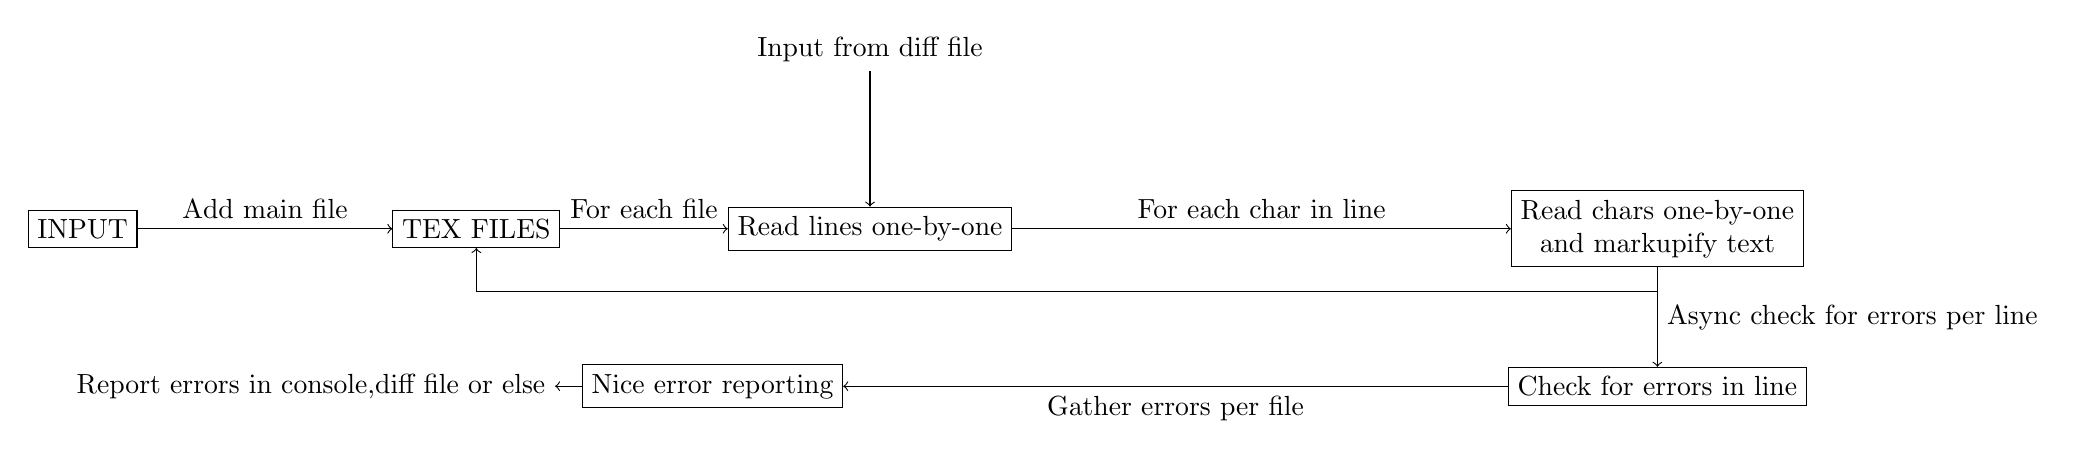
\begin{tikzpicture}
    \tikzstyle{block}=[draw,align=center]

    \node[block] (input) at (0,0) {INPUT};
    \node[block] (files) at (5,0) {TEX FILES};
    \node[block] (read_lines) at (10,0) {Read lines one-by-one};
    \node[block] (read_chars) at (20,0) {Read chars one-by-one\\ and markupify text};
    \node[block] (server) at (20,-2) {Check for errors in line};
    \node[block] (reporting) at (8, -2) {Nice error reporting};

    \draw[->] (input) -- (files) node[midway,above] {Add main file};
    \draw[->] (files) -- (read_lines) node[midway,above] {For each file};
    \draw[->] (read_lines) -- (read_chars) node[midway,above] {For each char in line};
    \draw[->] (read_chars) -- (server) node[midway,right] {Async check for errors per line};
    \draw[->] (server) -- (reporting) node[midway,below] {Gather errors per file};
    \draw[->] (reporting) -- ++(-2,0) node[left] {Report errors in console,\\ diff file or else};
    \draw[<-] (read_lines) -- ++(0,2) node[above] {Input from diff file};
    \draw[->] (read_chars.south) -| ++(0,-.3) -| (files);
\end{tikzpicture}
\end{document}
